\section{Einleitung}

Willkommen auf deiner Reise durch die Analysis! Dieses Fachgebiet der Mathematik ist unglaublich mächtig und hilft uns, Veränderungen zu verstehen und zu beschreiben – von der Geschwindigkeit eines Autos bis zum Wachstum einer Pflanze. Bevor wir uns aber in die Tiefen der Differential- und Integralrechnung stürzen, wollen wir mit einigen Grundlagen beginnen, die du vielleicht schon aus früheren Schuljahren kennst. Diese Grundlagen sind das Fundament, auf dem alles Weitere aufbaut.

\begin{merksatzumgebung}[Zielsetzung]{Was erwartet dich hier?}
Dieses Lernmaterial ist dein Begleiter auf einer Reise durch wichtige Bereiche der Mathematik. Wir starten ganz einfach mit dem \textbf{Dreisatz}, den du vielleicht schon kennst. Von dort aus bauen wir unser Wissen Schritt für Schritt auf: Wir lernen \textbf{Funktionen} kennen, schauen uns an, wie sie sich verändern (\textbf{Differentialrechnung}) und wie wir Flächen unter ihnen berechnen können (\textbf{Integralrechnung}). Du wirst sehen, wie diese Ideen zusammenhängen und wofür man sie braucht.
Dieses Material soll dir auch einen guten Überblick über Themen geben, die im \textbf{Abitur in NRW} wichtig sind.
\end{merksatzumgebung}

Es ist wichtig zu verstehen, dass Mathematik nicht nur aus isolierten Themen besteht. Vielmehr bauen die Konzepte aufeinander auf und sind miteinander verwoben wie ein großes Netz. Der Dreisatz zum Beispiel ist eine einfache Form proportionaler Zusammenhänge, die uns direkt zu den linearen Funktionen führen. Und das Verständnis linearer Funktionen ist unerlässlich, bevor wir uns komplexeren Funktionstypen zuwenden.

\begin{infoboxumgebung}{Wichtiger Hinweis und Voraussetzungen}
Die Mathematik ist ein riesiges Feld! In deinen Schulbüchern findest du noch viele weitere spannende Themen. Dieses Material hier ist ein guter Anfang und soll dir die wichtigsten Grundlagen der Analysis erklären. Es ist nicht alles, was es gibt, aber es ist ein starkes Fundament, auf dem du aufbauen kannst.

\textbf{Für wen ist dieses Material gedacht und was solltest du mitbringen?}
Dieses Material ist für Alle gedacht, die sich im Selbststudium oder begleitend zum Unterricht in die Analysis einarbeiten möchten. Die Sprache ist Deutsch. Wenn Deutsch nicht deine Muttersprache ist, versuche, die mathematischen Begriffe und die Erklärungen langsam zu lesen. Mathematik hat oft ihre eigene 'Sprache' mit Symbolen, die überall auf der Welt gleich sind! Nutze vielleicht auch ein Wörterbuch für Fachbegriffe.

Um gut mit diesem Skript arbeiten zu können, solltest du einige grundlegende mathematische Fähigkeiten mitbringen:
\begin{itemize}
    \item \textbf{Lineare Gleichungen umformen:} Du solltest sicher im Umstellen von einfachen Gleichungen nach einer Unbekannten sein (Äquivalenzumformungen).
    \item \textbf{Bruchrechnung:} Das Addieren, Subtrahieren, Multiplizieren und Dividieren von Brüchen sollte dir vertraut sein.
    \item \textbf{Grundlegende algebraische Regeln:} Dazu gehören das Ausmultiplizieren von Klammern, das Anwenden der binomischen Formeln und das Rechnen mit Potenzen und Wurzeln. Viele dieser Aspekte werden wir zwar wiederholen, aber eine gewisse Grundsicherheit ist hilfreich.
\end{itemize}
Keine Sorge, wenn nicht alles perfekt sitzt! Dieses Skript ist so aufgebaut, dass viele Konzepte von Grund auf erklärt werden. Für eine detailliertere Übersicht über algebraische Grundlagen wird es eventuell eine separate Formelsammlung oder ein Grundlagenkapitel geben. Wichtig ist deine Bereitschaft, dich aktiv mit den Inhalten auseinanderzusetzen.
\end{infoboxumgebung}

\begin{funfactbox}{Die geheimen Lieblingszahlen der Natur?}
Hast du schon einmal die Spiralen auf einem Tannenzapfen gezählt oder die Anordnung der Kerne in einer Sonnenblume genauer betrachtet? Oft verbirgt sich dahinter eine faszinierende Zahlenfolge, die als \textbf{Fibonacci-Folge} bekannt ist!

Sie beginnt ganz einfach mit 1 und 1 (manchmal auch mit 0 und 1), und jede weitere Zahl ist die Summe ihrer beiden Vorgänger:
\[ 1, 1, 2, 3, 5, 8, 13, 21, 34, 55, \dots \]
(Denn $1+1=2$, $1+2=3$, $2+3=5$, und so weiter.)

Das Erstaunliche: Diese Zahlen tauchen unglaublich oft in der Natur auf!
\begin{itemize}
    \item Die Anzahl der Blütenblätter vieler Blumen ist eine Fibonacci-Zahl (z.B. Lilien haben oft 3, Butterblumen 5, Astern 21 oder 34).
    \item Die Spiralen bei Tannenzapfen, Ananas oder den Kernen von Sonnenblumen verlaufen oft in Anzahlen, die benachbarte Fibonacci-Zahlen sind.
    \item Auch bei der Verzweigung von Bäumen oder der Anordnung von Blättern an einem Stiel findet man manchmal diese Muster.
\end{itemize}
Es ist, als ob die Natur eine Vorliebe für diese Zahlenfolge hätte, weil sie effizientes Wachstum und eine optimale Anordnung ermöglicht.

\textbf{Noch eine Verblüffung (ein kleiner Ausblick):} Wenn du aufeinanderfolgende Zahlen der Fibonacci-Folge durcheinander teilst (z.B. $8/5 = 1,6$; $13/8 = 1,625$; $21/13 \approx 1,61538$; $34/21 \approx 1,61904$), nähern sich die Ergebnisse immer mehr einer ganz besonderen irrationalen Zahl, dem \textbf{Goldenen Schnitt} $\Phi \approx 1,61803\dots$. Dieser Wert gilt seit der Antike als Inbegriff von Ästhetik und Harmonie in Kunst und Architektur!

Die Mathematik ist voller solcher überraschender Muster und Querverbindungen, die uns helfen, die Struktur und Schönheit der Welt um uns herum – und in der Mathematik selbst – zu entdecken. Dieses Buch ist eine Einladung, einige weitere dieser faszinierenden Zusammenhänge aufzuspüren!

\begin{center}
    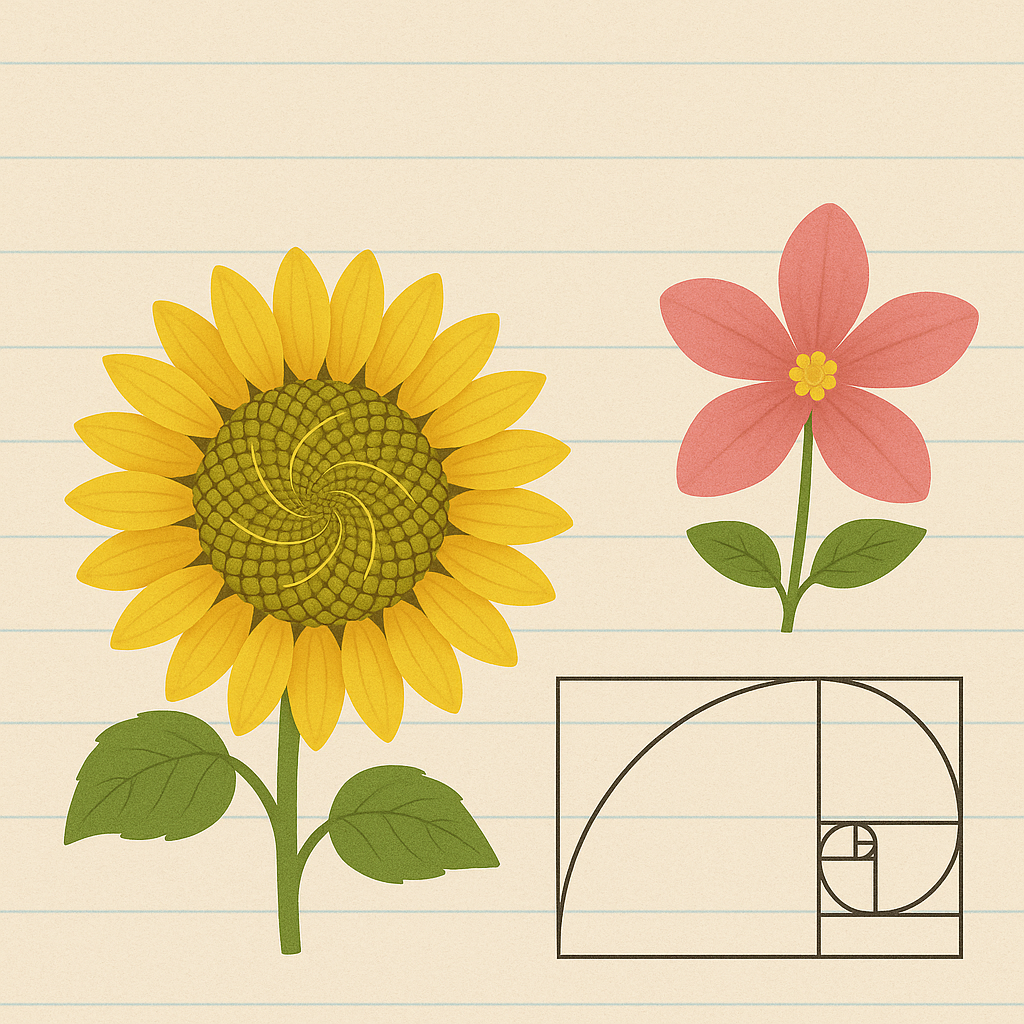
\includegraphics[width=0.5\textwidth]{grafiken/Fibonacci_Natur_Collage.png}
    % Beschreibung für die Grafik 'Fibonacci_Natur_Collage.png':
    % Die Grafik könnte eine ansprechende Collage sein, die einige der genannten Beispiele zeigt:
    % - Eine Sonnenblume mit deutlich sichtbaren Spiralen in den Kernen.
    % - Eine Blüte mit einer Fibonacci-Anzahl an Blütenblättern (z.B. eine mit 5 oder 8).
    % - Die ersten Zahlen der Fibonacci-Folge: 1, 1, 2, 3, 5, 8...
    % - Eventuell eine stilisierte Fibonacci-Spirale (die sich aus aneinandergereihten Quadraten 
    %   mit Fibonacci-Seitenlängen ergibt).
    \captionof{figure}{Fibonacci-Zahlen und der Goldene Schnitt offenbaren Muster in der Natur.}
    \label{fig:fibonacci_natur_funfact}
\end{center}
\end{funfactbox}